% Define block styles
\tikzstyle{block} = [draw, rectangle, text centered, text width=5cm, minimum height=1cm, rounded corners=true]
\tikzstyle{arrowtext} = [text width=4em, text centered]
\tikzstyle{arrow} = [draw, -latex]

\definecolor{red1}{RGB}{160,0,0}
\definecolor{green1}{RGB}{0,160,0}
\definecolor{blue1}{RGB}{0,0,160}

	      
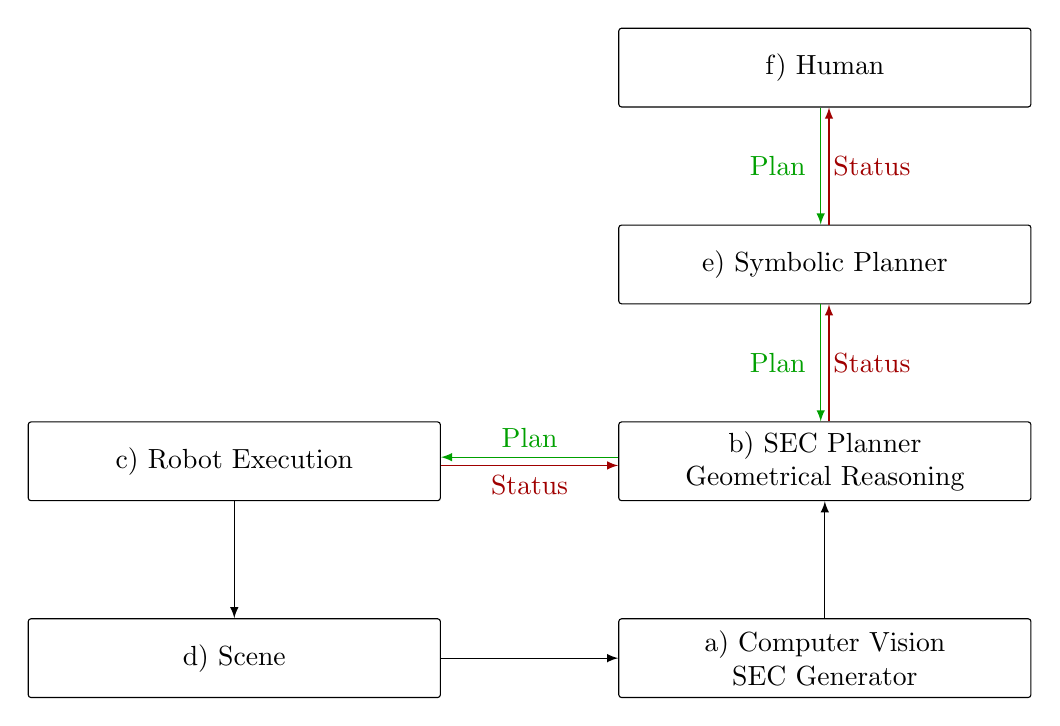
\begin{tikzpicture}[node distance=2.5cm, auto]
	\node [block] (scene) {d) Scene};
	\node [block, right of=scene, node distance=7.5cm] (computervision) {a) Computer Vision\\SEC Generator};
	\node [block, above of=computervision] (planner_sec) {b) SEC Planner\\Geometrical Reasoning};
	\node [block, above of=planner_sec] (planner_highlevel) {e) Symbolic Planner};
	\node [block, above of=planner_highlevel] (planner_human) {f) Human};
	\node [block, above of=scene] (robot) {c) Robot Execution};

	\draw [arrow] (robot.south) to (scene.north);
	\draw [arrow] (scene.east) to (computervision.west);
	\draw [arrow] (computervision.north) to (planner_sec.south);

	% Planner SEC
	\draw [arrow, color=green1] ([yshift=0.15em] planner_sec.west) to node[arrowtext, above, name=plan] {Plan} ([yshift=0.15em] robot.east);
	\draw [arrow, color=red1] ([yshift=-0.15em] robot.east) to node[arrowtext, below, name=error] {Status} ([yshift=-0.15em] planner_sec.west);

	% High level
	\draw [arrow, color=red1] ([xshift=0.15em] planner_sec.north) to node[arrowtext, right, name=error, xshift=-0.8em] {Status} ([xshift=0.15em] planner_highlevel.south);
	\draw [arrow, color=green1] ([xshift=-0.15em] planner_highlevel.south) to node[arrowtext, left, name=plan, xshift=0.8em] {Plan} ([xshift=-0.15em] planner_sec.north);

	% Human
	\draw [arrow, color=red1] ([xshift=0.15em] planner_highlevel.north) to node[arrowtext, right, name=error, xshift=-0.8em] {Status} ([xshift=0.15em] planner_human.south);
	\draw [arrow, color=green1] ([xshift=-0.15em] planner_human.south) to node[arrowtext, left, name=plan, xshift=0.8em] {Plan} ([xshift=-0.15em] planner_highlevel.north);
\end{tikzpicture}
